% User guide

The developed plugin is fully usable from either the command line, or the GUI. It's also possible to mix and match the two, for example it would be fine to install the plugin using the CLI and then use it with the GUI. This section is mainly split into two subsections for clarity.

\subsection{CLI}

Provided that the installed \textit{weka.jar} file is on the classpath, the following examples should be reproducible on any system. If the \textit{weka.jar} file is not on the class path, then the -cp flag must also be appended to the command. For example:

\begin{footnotesize}
\begin{verbatim}
java weka.classifiers.bayes.NaiveBayes -t training.arff
\end{verbatim}
\end{footnotesize}
would have to become
\begin{footnotesize}
\begin{verbatim}
java -cp /home/path/to/jar/weka.jar weka.classifiers.bayes.NaiveBayes
        -t training.arff
\end{verbatim}
\end{footnotesize}

The plugin can be installed using Weka's package manager using the following command, assuming that the cdc04 zip file is in the current directory:

\begin{footnotesize}
\begin{verbatim}
java weka.core.WekaPackageManager -install-package cdc04.zip
\end{verbatim}
\end{footnotesize}

An example of using the classifier from the command line would be:

\begin{footnotesize}
\begin{verbatim}
java weka.Run ProjectClassifier -t audiology.arff
        -W weka.classifiers.bayes.NaiveBayes -S -M 30 -- -O
\end{verbatim}
\end{footnotesize}

Any parameters which follow the \textit{- -} are passed to the target classifier. If there is any doubt about flags or parameters, use the help flag (-h).

\subsection{GUI}

Once Weka is running the plugin can be imported using the package manager which can be found in the menu shown in Figure \ref{main}.
\begin{figure}[ht!]
\centering
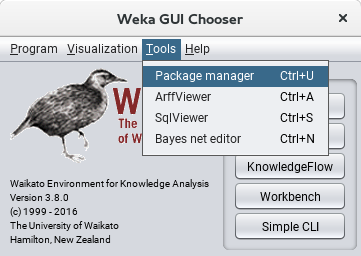
\includegraphics[width=70mm]{weka_main_screen.png}
\caption{Weka Main Menu \label{main}}
\end{figure}

This will bring up the screen shown in \ref{package_man}. The plugin can be installed by clicking the \textit{File/Url} button in the top right corner, and then adding the \textit{cdc04.zip} file.

\begin{figure}[ht!]
\centering
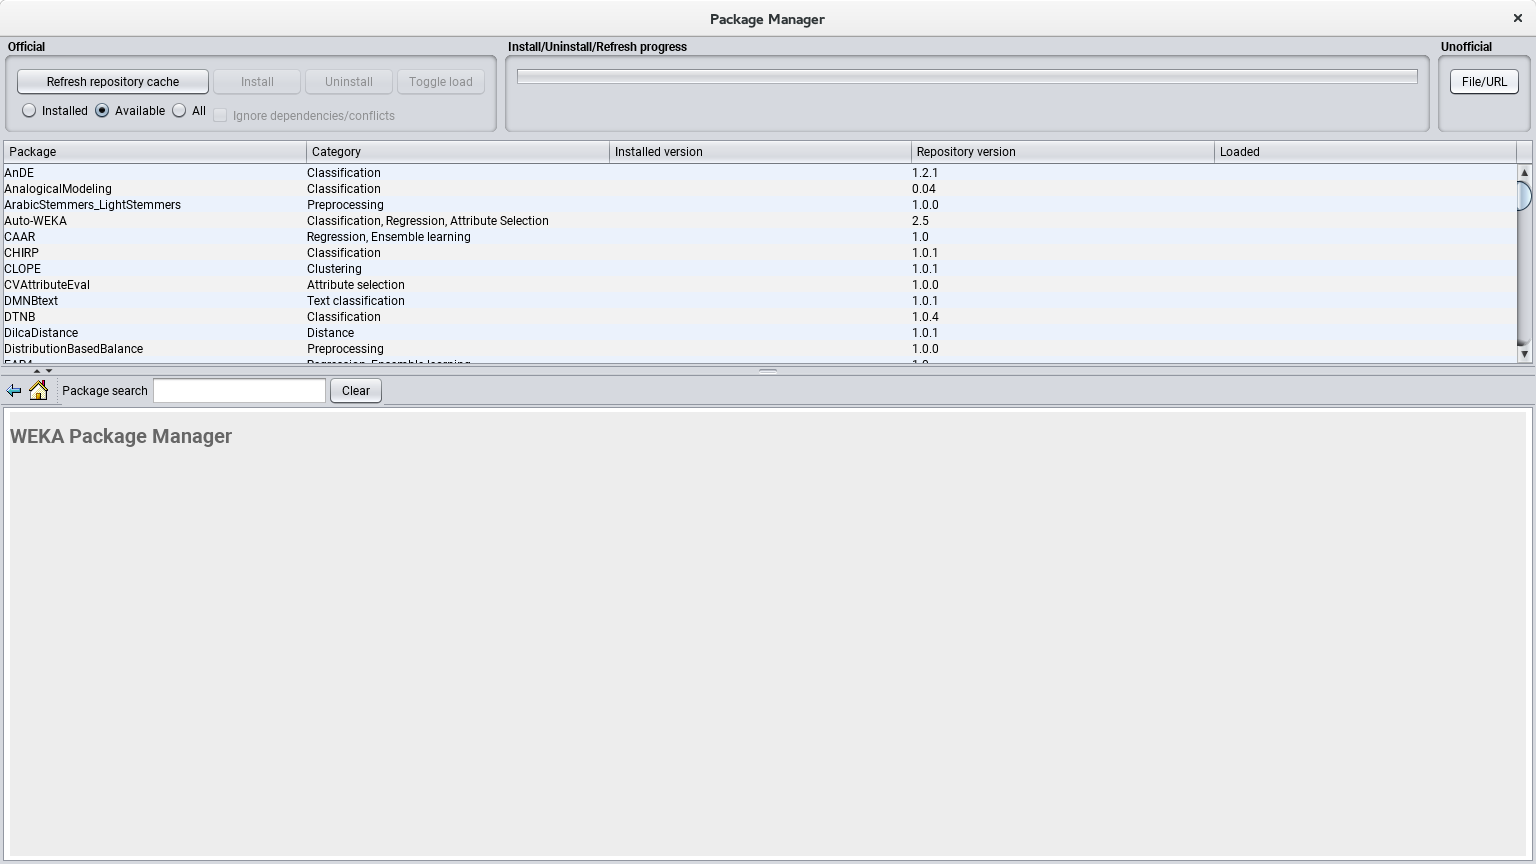
\includegraphics[width=160mm]{package_manager.png}
\caption{Weka Package Manager \label{package_man}}
\end{figure}

Once the plugin has been installed, it can then be used throughout Weka. For example in the explorer it can be found under \textit{Weka / Classifiers / Meta} as shown in Figure \ref{explore_classify}.

\begin{figure}[ht!]
\centering
    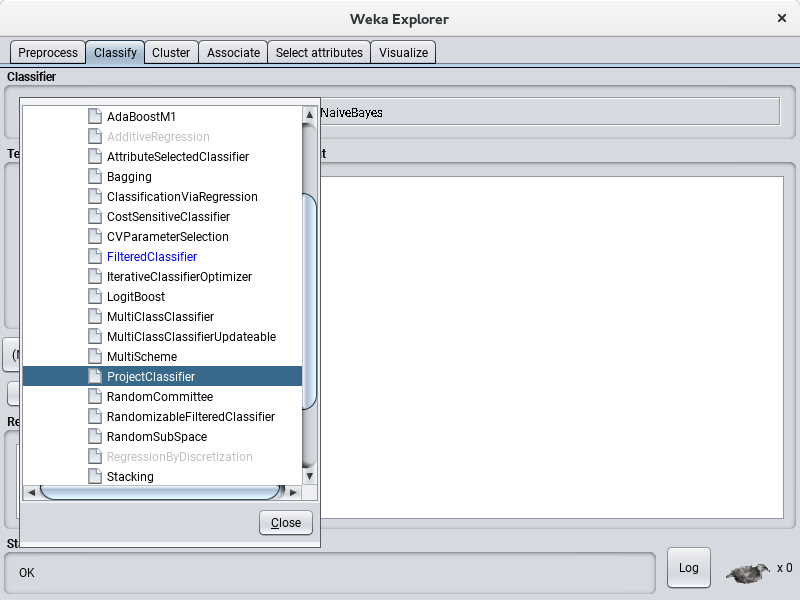
\includegraphics[width=120mm]{explore_classify.png}
\caption{Weka Classifier Selector \label{explore_classify}}
\end{figure}

This can then be configured using the interface shown in Figure \ref{project_classifier_gui}. Clicking the name of the internal classifier will allow it to be configured using its own, similar window.

\begin{figure}[ht!]
\centering
    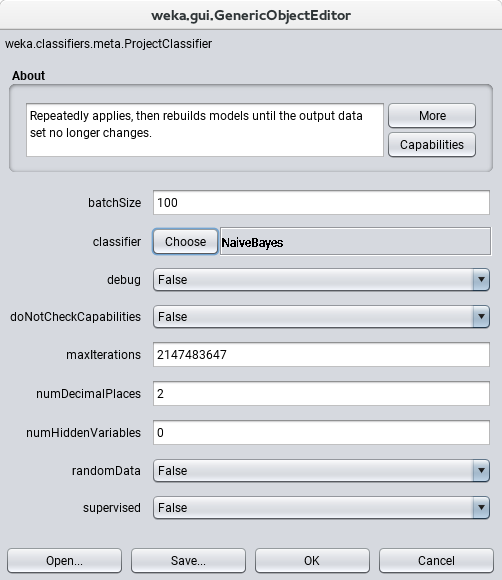
\includegraphics[width=100mm]{project_classifier_interface.png}
\caption{Project Classifier Configuration GUI \label{project_classifier_gui}}
\end{figure}


